\documentclass[10pt]{beamer}

%%%
% GENERAL PREAMBLE
%%%
%https://tex.stackexchange.com/questions/68821/is-it-possible-to-create-a-latex-preamble-header
\usepackage{/Users/miw267/Repos/latex_preamble/beamer_preamble}


% FOR THIS DECK
\usetikzlibrary{arrows.meta, positioning}


\agendatopic[quiz]{Quizzes: Extra Credit Quiz and Quiz Review}
\agendatopic[pgm]{Probabilistic Graphical Models}
\agendatopic[connection]{Connection}

%%%
% DOCUMENT
%%%

\begin{document}





\title{11/18/2026: Connection}
\author{CSCI 246: Discrete Structures}
\date{Textbook reference: Lov\'asz Sec 7.2}

\begin{frame}
    \titlepage 
\end{frame}

\begin{frame}
\begin{mygreenbox}[title=Graded Quiz Pickup]
Quizzes are in the front of the room, grouped into four bins (A-G, H-L, M-R, S-Z) by last name. The quizzes are upside down with your last name on the back. Come find yours before, during, or after class. Only turn the quiz over if it's yours. 
\end{mygreenbox} 
\vfill 
\begin{myredbox}[title=\text{Announcements}]
Reminder: Readings for Graph Theory Module have changed. See syllabus.
\end{myredbox}

\vfill 
\begin{myyellowbox}[title=Today's Agenda]
\begin{itemize}
	\item Extra credit quiz (5 mins)
	\item Review quizzes ($\approx$ 10 mins)
	\item Mini-lecture: Probabilistic Graphical Models ($\approx$ 15 mins)
	\item Mini-lecture: Connection ($\approx$ 10 mins)
	\item New group exercises ($\approx$ 10 mins)
\end{itemize}


\end{myyellowbox}
\vfill 

\end{frame}


\agendaframe{quiz}


\begin{frame}

\begin{mygreenbox}[title=\text{Extra Credit Reading Quiz (Lov\'asz Sec 7.1)}]
Describe, at a high level, how you would prove the following theorem. Your answer should be between 1 and 3 sentences. \\

\vspace{.4cm}

\textbf{Theorem.} \textit{In every graph, the number of vertices with odd degree is even.}  
\end{mygreenbox}
		
\end{frame}


\begin{frame}[standout]
Extra Credit Reading Quiz: Review Solution
\\
\small
\vfill \vfill \vfill \vfill \vfill 
(See the solution to Group Exercise \#6 in the slides from 11/16, \textit{Fundamentals of Graph Theory.})
\end{frame}



\begin{frame}{Alternative Solution}

\begin{mygreenbox}[title=Handshake Lemma (Scheinerman Thm 47.5)]
Let $G=(V,E)$.  The sum of the degrees of the vertices in $G$ is twice the number of edges; that is
\[ \sum_{v \in V} d(v) = 2 |E| \]
\end{mygreenbox}
\vfill 
\colorbox{blue!30}{\textbf{Remark.}} This theorem is very useful. For example, it could be used to realize Izayah (Fall 2025)'s idea to prove the theorem by contradiction (rather than by induction).  See Lov\'asz pp. 130.
\end{frame}



\begin{frame}[standout]
Quiz \#10 Results
\bottomtext{The 3-of-a-kind poker question was made extra credit.}
\end{frame}

\begin{frame}{Quiz \#10 Results}
\centering 
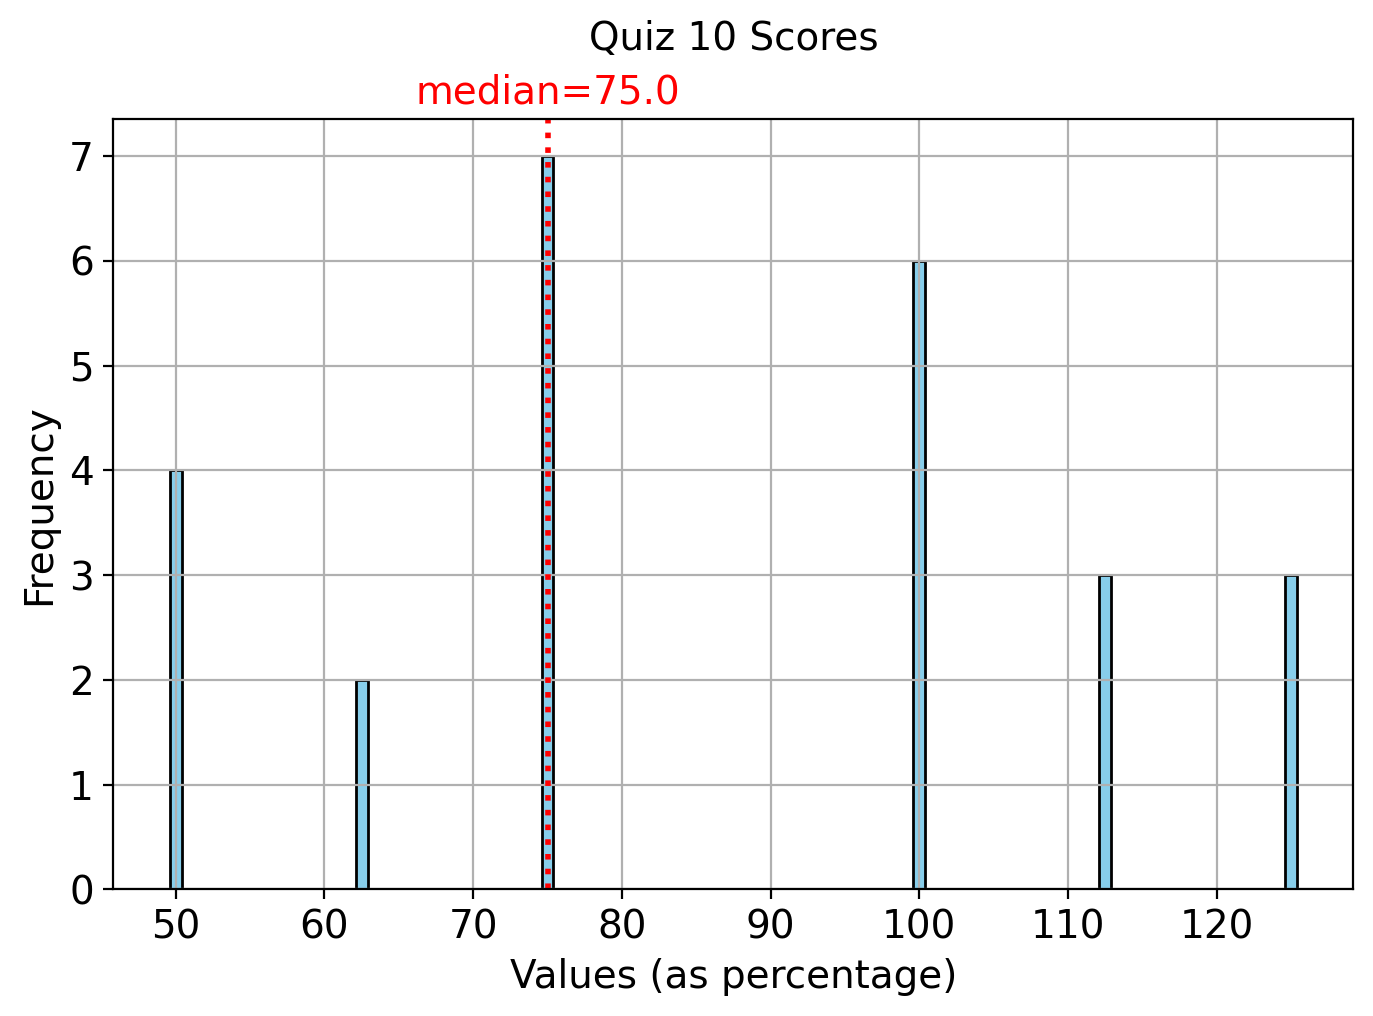
\includegraphics[width=.80\textwidth]{images/quiz_10_histogram.png}	
\end{frame}


\begin{frame}[t]{Solution: Three of a Kind}
\footnotesize
\setlength{\abovedisplayskip}{2pt}
\setlength{\belowdisplayskip}{2pt}

\colorbox{blue!30}{\textbf{Problem.}} What is the probability of getting a \textbf{three of a kind} in a 5-card poker hand?

\colorbox{green!30}{\textbf{Solution.}} Let $S$ be the set of all 5-card poker hands, and let $E \subset S$ be the three of a kind hands.  By the equally likely probability formula,
\[
P(E) = \frac{|E|}{|S|} = \frac{\text{\# of three of a kind poker hands}}{\text{\# of poker hands}} = \frac{|E|}{\binom{52}{5}} = \frac{|E|}{2{,}598{,}960}.
\]
So we just need to find $|E|$.  We build a hand in steps:

% five cards, filled in as the steps are revealed
\vspace{-0.1cm}
\begin{center}
\begin{tikzpicture}[card/.style={draw, rounded corners=2pt, minimum width=0.65cm, minimum height=0.7cm, font=\normalsize}]
  \node[card] at (0,0)    {\only<2->{K}\only<3->{$\spadesuit$}};
  \node[card] at (0.85,0) {\only<2->{K}\only<3->{\textcolor{red}{$\heartsuit$}}};
  \node[card] at (1.7,0)  {\only<2->{K}\only<3->{\textcolor{red}{$\diamondsuit$}}};
  \node[card] at (2.9,0)  {\only<4->{7}\only<5->{$\clubsuit$}};
  \node[card] at (3.75,0) {\only<4->{2}\only<5->{\textcolor{red}{$\heartsuit$}}};
\end{tikzpicture}
\end{center}

\vspace{-0.5cm}
\begin{enumerate}\setlength{\itemsep}{0pt}
  \item<2-> \textbf{Choose a rank} for the three of a kind: \hfill $13$ choices
  \item<3-> \textbf{Choose three suits} for the three of a kind: \hfill $\binom{4}{3} = 4$ choices
  \item<4-> \textbf{Choose two ranks} for the kickers (from the other 12): \hfill $\binom{12}{2} = 66$ choices
  \item<5-> \textbf{Choose a suit} for each kicker: \hfill $4 \times 4 = 16$ choices
\end{enumerate}

\onslide<6->{\alert{\textbf{Final Answer.}} $|E| = 13 \cdot 4 \cdot 66 \cdot 16 = 54{,}912$, so $P(E) = \frac{54{,}912}{2{,}598{,}960} \approx 0.021$ (1 in 47).}

\vspace{0.1cm}
\onslide<7->{\colorbox{red!30}{\textbf{Note.}} Many students did step 3 as $12 \times 11$.  But that assumes order matters, counting (7, 2) and (2, 7) as different hands.  Note that $\binom{12}{2} = \frac{12 \times 11}{2}$, which automatically corrects for order.}
\end{frame}



\begin{frame}[standout]
Study Guide For Quiz \#11
\end{frame}



\begin{frame}{Study Guide For Quiz \#11}
\scriptsize 

\colorbox{yellow!20}{\textbf{Group exercises.}} Know how to solve the group exercises from the course meetings on Random Variables (11/9), Expectation and Variance (11/13), and Graph Theory Fundamentals (11/16).

\vfill 
\colorbox{red!20}{\textbf{Readings.}}    Scheinerman Sec. 33 (Random variables)
\vspace{-.2cm}
\begin{itemize}
\item Know the definition of a random variable (Def 33.1), as applied in Examples 33.2-33.4.
\item Know how to determine whether two random variables are independent (see Def 33.6, as well as the preceding discussion).
\end{itemize}


Scheinerman Sec. 34 (Expectation and Variance)
\vspace{-.2cm}
\begin{itemize}
\item Know how to \textbf{compute the expectation} according to Def 34.1 (see Examples 34.1 and 34.2) and according to Prop 34.4 (see Examples 34.5 and 34.6).
\item Know these two results: \textbf{linearity of expectation} (Theorem 34.10) and the \textbf{expectation of a product} of independent random variables (Theorem 34.14). Also know how to apply these to concrete problems.
\item Know how to \textbf{compute the variance} according to Def 34.16 (see Examples 34.17 and 34.18) and according to Prop 34.19 (see Example 34.20). 
\end{itemize}

Scheinerman Sec. 47 (Fundamentals of Graph Theory)
\vspace{-.2cm}
\begin{itemize}
\item Know the definitions of a \textbf{graph} (Def 47.1), \textbf{adjacency} (Def 47.3), and \textbf{degree} (Def 47.4). 
\item Know \textbf{Theorem 47.5}: its result and how to defend it. (1-2 sentences suffices.)
\end{itemize}

\end{frame}


\agendaframe{pgm}



\begin{frame}[standout]
Probabilistic Graphical Models
\\
\small
\vfill \vfill \vfill \vfill \vfill 
(See the section in the slides from 11/16, \textit{Fundamentals of Graph Theory.})
\end{frame}



\agendaframe{connection}



\begin{frame}{Walks vs. Paths}
\small
\begin{minipage}[t]{0.50\textwidth}
\centering
\vspace{0pt}
{\large \alert{\textbf{Walk}}} \\[0.1cm]
A walk is a sequence of vertices, with each vertex adjacent to the next. \\[0.2cm]
{\small \textbf{Example.}  $A \sim B \sim C \sim B \sim C \sim D \sim E$.} \\[0.2cm]

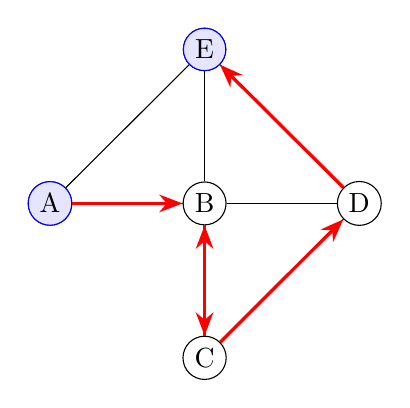
\begin{tikzpicture}[node distance=1.4cm, every node/.style={circle, draw, inner sep=2pt, minimum size=5mm}]
  \node (A) {A};
  \node (B) [right=of A] {B};
  \node (C) [below=of B] {C};
  \node (D) [right=of B] {D};
  \node (E) [above=of B] {E};

  % base edges
  \draw (A) -- (B);
  \draw (B) -- (C);
  \draw (B) -- (D);
  \draw (B) -- (E);
  \draw (C) -- (D);
  \draw (A) -- (E);
  \draw (D) -- (E);

  % highlight start/end
  \node[draw=blue, fill=blue!10, circle, inner sep=2pt, minimum size=5mm] at (A) {A};
  \node[draw=blue, fill=blue!10, circle, inner sep=2pt, minimum size=5mm] at (E) {E};

  % highlighted walk (repeats allowed)
  \draw[very thick, red, -{Stealth}] (A) -- (B);
  \draw[very thick, red, -{Stealth}] (B) -- (C);
  \draw[very thick, red, -{Stealth}] (C) -- (B);
  \draw[very thick, red, -{Stealth}] (C) -- (D);
  \draw[very thick, red, -{Stealth}] (D) -- (E);
\end{tikzpicture}
\end{minipage}%
\hfill
\begin{minipage}[t]{0.40\textwidth}
\centering
\vspace{0pt}
{\large \alert{\textbf{Path}}} \\[0.1cm]
A path is a walk in which no vertex is repeated. \\[0.2cm]
{\small \textbf{Example.} $A \sim B \sim C \sim D \sim E$.}\\[0.2cm]

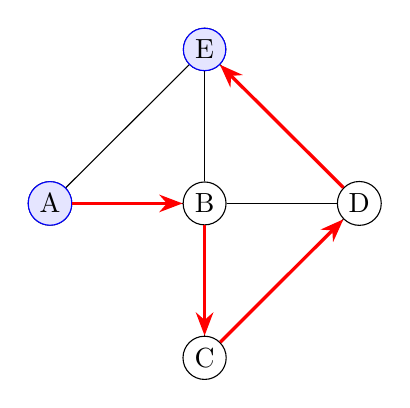
\begin{tikzpicture}[node distance=1.4cm, every node/.style={circle, draw, inner sep=2pt, minimum size=5mm}]
  \node (A) {A};
  \node (B) [right=of A] {B};
  \node (C) [below=of B] {C};
  \node (D) [right=of B] {D};
  \node (E) [above=of B] {E};

  
  % base edges
  \draw (A) -- (B);
  \draw (B) -- (C);
  \draw (B) -- (D);
  \draw (B) -- (E);
  \draw (C) -- (D);
  \draw (A) -- (E);
  \draw (D) -- (E);

  % highlight start/end
  \node[draw=blue, fill=blue!10, circle, inner sep=2pt, minimum size=5mm] at (A) {A};
  \node[draw=blue, fill=blue!10, circle, inner sep=2pt, minimum size=5mm] at (E) {E};

  % highlighted path (no repeats)
  \draw[very thick, red, -{Stealth}] (A) -- (B);
  \draw[very thick, red, -{Stealth}] (B) -- (C);
  \draw[very thick, red, -{Stealth}] (C) -- (D);
  \draw[very thick, red, -{Stealth}] (D) -- (E);
\end{tikzpicture}
\end{minipage}
\pause 
\vfill 
\colorbox{yellow!30}{\textbf{Remark.}} A path is a subgraph:  \quad 
\includegraphics[width=3cm]{images/path_graph}
\end{frame}



\begin{frame}{\qq{Connected to}}
\footnotesize 
\begin{mygreenbox}[title=Definition]
Let $G$ be a graph and let $u,v \in V(G)$.  We say that $u$ is \textbf{connected to} $v$ provided that there is a $(u,v)$-path in $G$ (i.e., a path whose first vertex is $u$ and whose last vertex is $v$).	
\end{mygreenbox}
\vfill 
\begin{center}
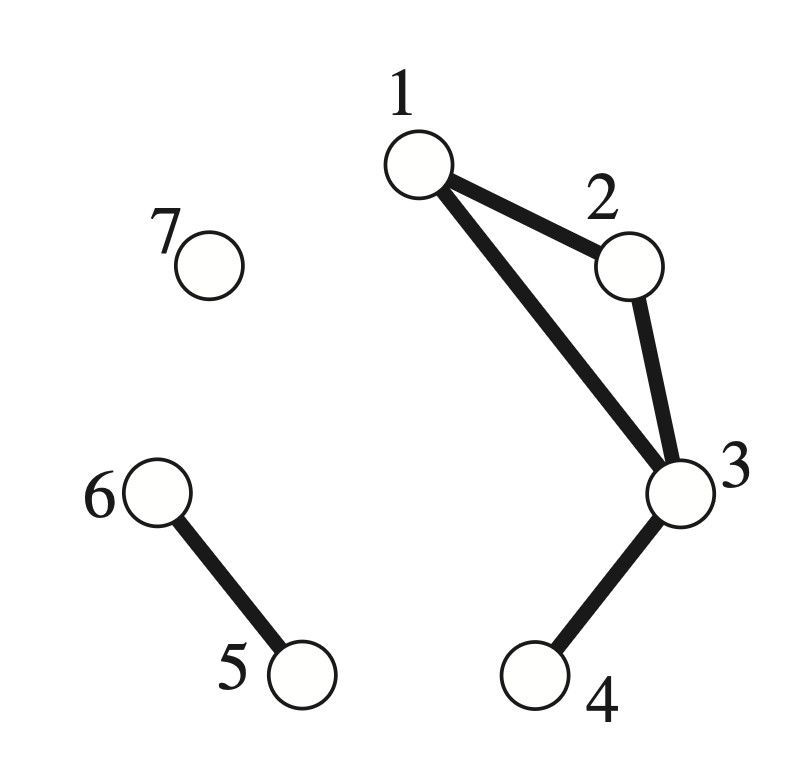
\includegraphics[width=.25\textwidth]{images/disconnected_graph}
\end{center}
\vfill 
\only<2>{\colorbox{yellow!30}{\textbf{Poll.}} What is the difference between \qq{connected to} and \qq{adjacent to}?}
\vfill 
\only<3->{\begin{myredbox}[title=Theorem]
Let $G$ be a graph.  The is-connected-to relation is an equivalence relation on $V(G)$.
\end{myredbox}
}
\vfill 
\only<4>{\colorbox{yellow!30}{\textbf{Poll.}} Who can talk us through why this is true, using the example above?}

%\only<5->{\colorbox{blue!30}{\textbf{Who cares?}}} \only<6->{This theorem forms the basis for efficient algorithms, like connected component labeling in image processing, or Kruskal’s algorithm (for minimum spanning trees).} 

\only<5->{\colorbox{blue!30}{\textbf{Who cares?}}} \only<6->{This theorem forms the basis for efficient algorithms for problems like \textit{dynamic connectivity}, the problem of answering \qq{can A reach B?} in a network that keeps changing.}
\end{frame}



\begin{frame}{Components}
\small 
\begin{mygreenbox}[title=Definition (Scheinerman Def 49.9)]
A \textbf{component} of a graph $G$ is a subgraph of $G$ induced on an equivalence class of the is-connected-to relation on $V(G).$
\end{mygreenbox}
\vfill 


\begin{center}
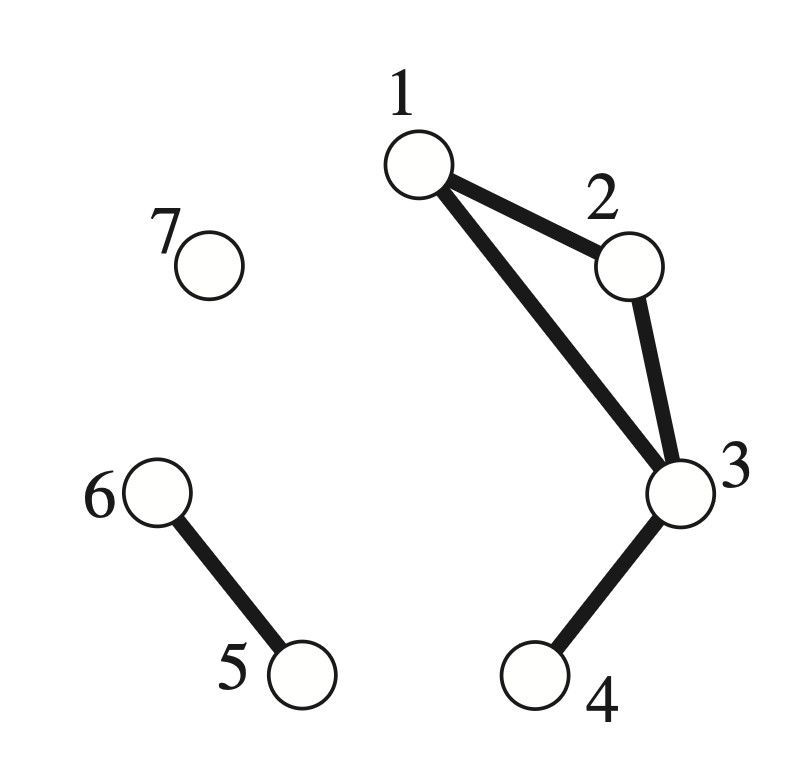
\includegraphics[width=.22\textwidth]{images/disconnected_graph}
\end{center}
\vfill 
\colorbox{yellow!30}{\textbf{Poll.}} What are the components in the graph above?
\vfill 
\pause 
\colorbox{green!30}{\textbf{Solution.}} There are 3 components: $C_1 = \set{1,2,3,4}, C_2=\set{5,6}, C_3=\set{7}.$

\pause 

\begin{mygreenbox}[title=Alternate Definition]
%A \textbf{component} of a graph $G$ is a maximal set of vertices that are all connected to each other by paths.
A \textbf{component} is a connected subgraph that is not part of any larger connected subgraph.
\end{mygreenbox}


\end{frame}



\begin{frame}{Connected Graphs}
	
\begin{mygreenbox}[title=Definition]
A graph $G$ is called \textbf{connected} provided each pair of vertices in the graph is connected by a path; that is, for all $x,y \in V(G)$, there is an $(x,y)$-path.
\end{mygreenbox}
\vfill 
\begin{minipage}[t]{0.45\textwidth}
\centering
\vspace{0pt}
{\large \alert{\textbf{Disconnected}}} \\[0.1cm]
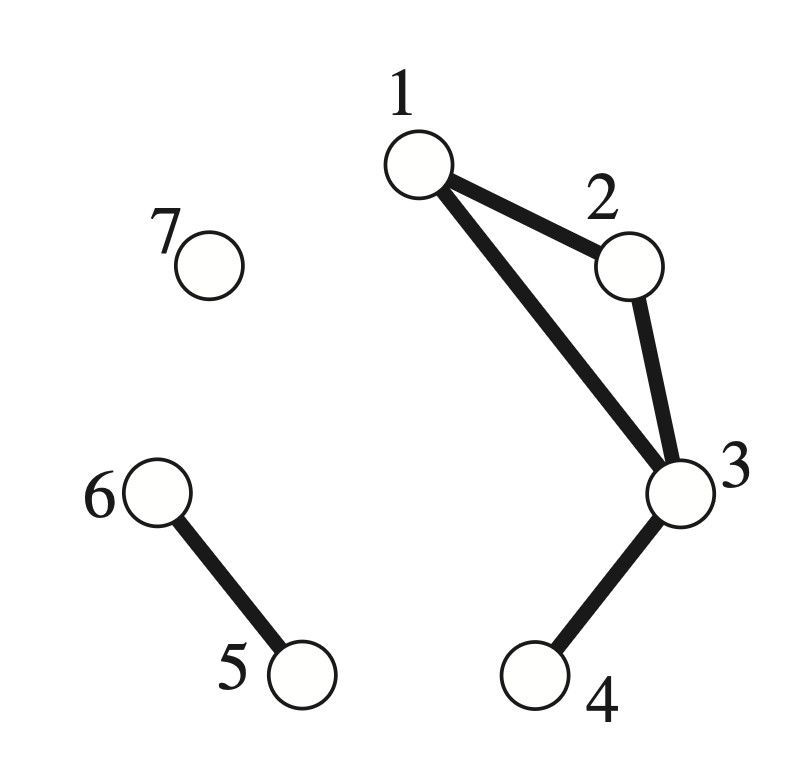
\includegraphics[width=.6\textwidth]{images/disconnected_graph.png}
\end{minipage}%
\hfill
\begin{minipage}[t]{0.45\textwidth}
\centering
\vspace{0pt}
{\large \alert{\textbf{Connected}}} \\[0.1cm]
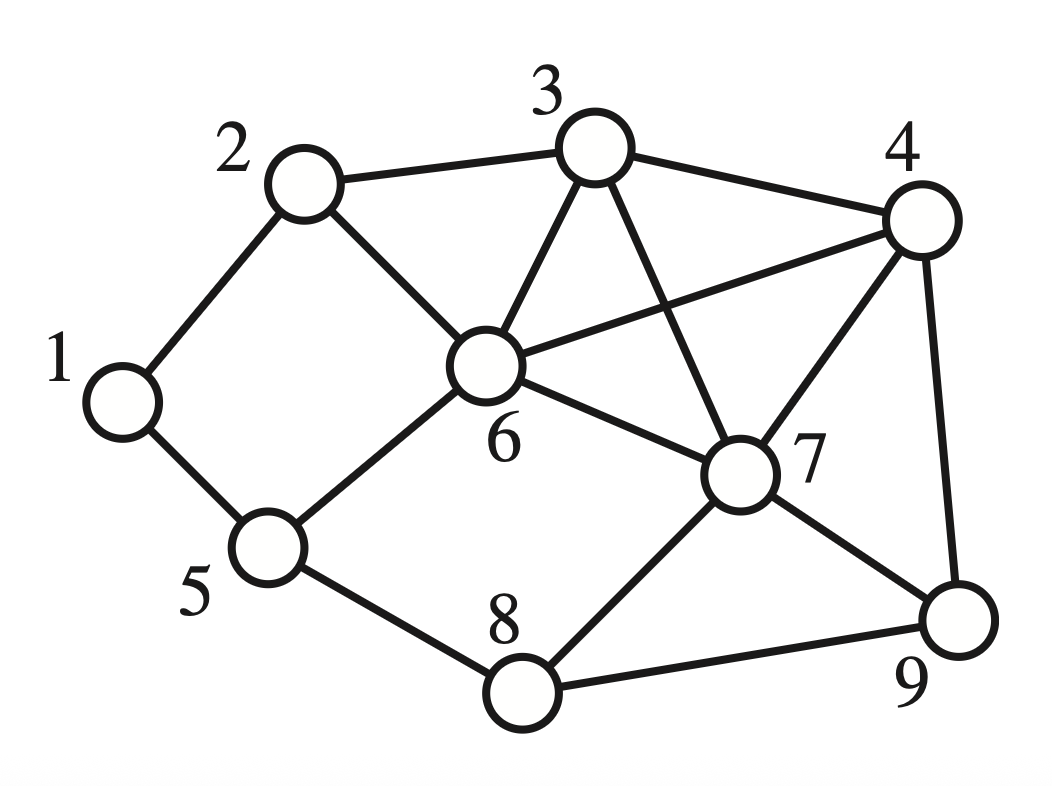
\includegraphics[width=.8\textwidth]{images/connected_graph.png}
\end{minipage}
\pause
\vfill
\colorbox{blue!30}{\textbf{Remark.}} $G$ is connected $\iff$ $G$ contains exactly 1 component.
\end{frame}


%\begin{frame}{Applications}
%
%\colorbox{red!30}{\textbf{Question.}} Why should I care that connected-to is an equivalence relation?
%
%\vfill 
%\pause 
%
%\colorbox{green!30}{\textbf{Answer (one of many).}} \textbf{Enables efficient algorithms (like Union–Find).}
%
%When you view connectedness as an equivalence relation, you can represent it using a \textbf{disjoint-set data structure (Union–Find).}
%
%\begin{itemize}
%\item Each equivalence class corresponds to a set (a connected component).
%\item \texttt{find}(x) gives the \qq{representative} of x’s component.
%\item \texttt{union}(x, y) merges components if an edge connects them.
%\end{itemize}
%
%
%\vfill 
%\pause 
%This is the basis for algorithms like:
%
%\begin{itemize}
%\item Kruskal’s algorithm (for minimum spanning trees),
%\item Connected component labeling in image processing,
%\item Dynamic connectivity maintenance in networks.	
%\end{itemize}
%
%\end{frame}
%






\begin{frame}[standout]
Group exercises
\end{frame}

\begin{frame}{Random Group Assignments}
%%% TABLE 1: by last name
\begin{columns}
\begin{column}{0.33\textwidth}
Ashley, Isabelle: 11 \\ 
Bailey, Tanna: 4 \\ 
Blaisdell, Olyver: 1 \\ 
Brown, Ashton: 9 \\ 
Cardenas, Dominic: 7 \\ 
Cutler, George: 11 \\ 
Fabik, Roland: 5 \\ 
Fuller, Ryan: 7 \\ 
Griffen, Clara: 11 \\ 
Grutsch, Tanner: 8 \\ 
Hager, Nathan: 2 \\\end{column}
\begin{column}{0.33\textwidth}
Horner, Jayden: 3 \\ 
Johnson, Jaret: 4 \\ 
Kintzel, Samantha: 1 \\ 
Lameres, Alexis: 4 \\ 
Lee, Holden: 6 \\ 
Mayala, Reece: 2 \\ 
McLean, Connor: 10 \\ 
Mcbride, Daniel: 5 \\ 
Miller, Maverick: 3 \\ 
Moss, Emily: 6 \\ 
Mousseau, Matthew: 6 \\\end{column}
\begin{column}{0.33\textwidth}
Neuman, Evan: 8 \\ 
Putnam, John: 3 \\ 
Rathbun, Jedidiah: 9 \\ 
Roberts, Matthew: 8 \\ 
Roller, Nathan: 9 \\ 
Ryan, Otis: 5 \\ 
Shevtsov, Timothy: 10 \\ 
Stensland, Emma: 2 \\ 
Thiessen, Logan: 7 \\ 
Thompson, Jaiden: 10 \\ 
Vath, Ethan: 1 \\\end{column}
\end{columns}
\end{frame}

\begin{frame}{Group exercises}
\small 
\noindent
\begin{minipage}{0.6\textwidth}
\begin{enumerate}
	\item  Let $G$ be the graph in the top figure.   (a) How many different paths are there from $a$ to $b$? (b) How many different walks are there from $a$ to $b$?
	\item Let $G$ be a graph.  A path $P$ in $G$ that contains all the vertices of $G$ is called a \textit{Hamiltonian Path}.  Prove that the graph in the bottom figure does not have a Hamiltonian path.
    \item How many Hamiltonian paths does a complete graph on $n \geq 2$ vertices have?
    \item Let $G$ be a graph with $n \geq 2$ vertices.  
    \begin{itemize}
    \item[a.] Prove that if G has at least $\binom{n-1}{2} +1$ edges, then $G$ is connected.
    \item[b.] Show that the result in (a) is best possible; that is, for each $n \geq 2$, prove there is a graph with 	$\binom{n-1}{2}$ edges that is not connected.
    \end{itemize}

\end{enumerate}
\end{minipage}%
\hfill
\begin{minipage}{0.38\textwidth}
   
    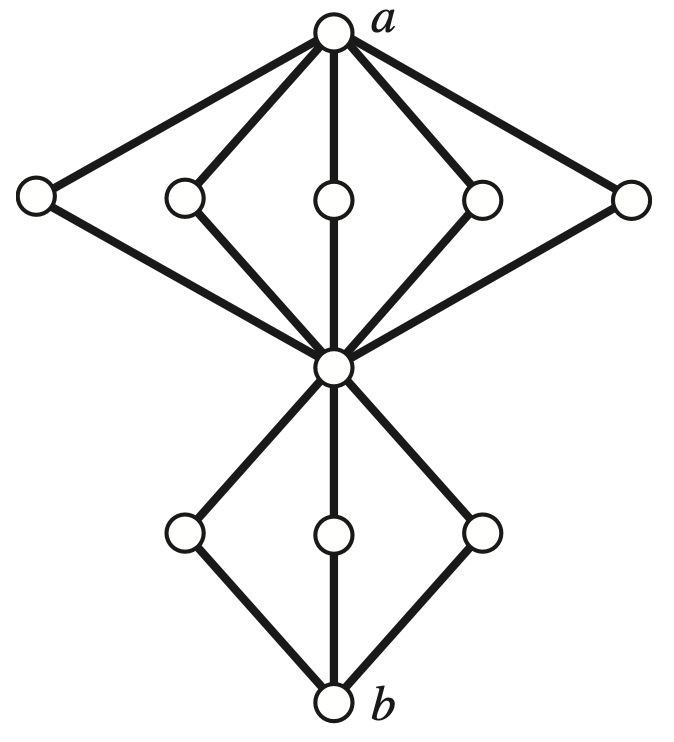
\includegraphics[width=\textwidth]{images/connection_exercise_1} %
    
    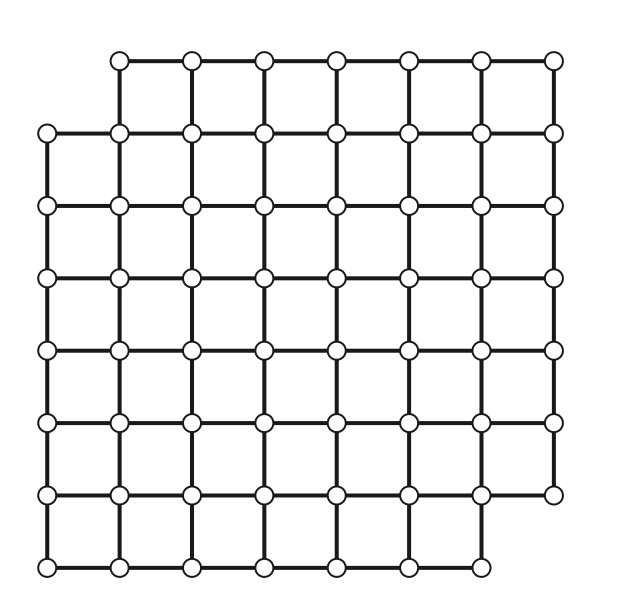
\includegraphics[width=\textwidth]{images/connection_exercise_2}
  
\end{minipage}%    

\end{frame}

\begin{frame}{Solution to group exercise \#1}
\small 
\noindent
\textbf{Problem.} Let $G$ be the graph in the top figure.   (a) How many different paths are there from $a$ to $b$? (b) How many different walks are there from $a$ to $b$?

\begin{center}
    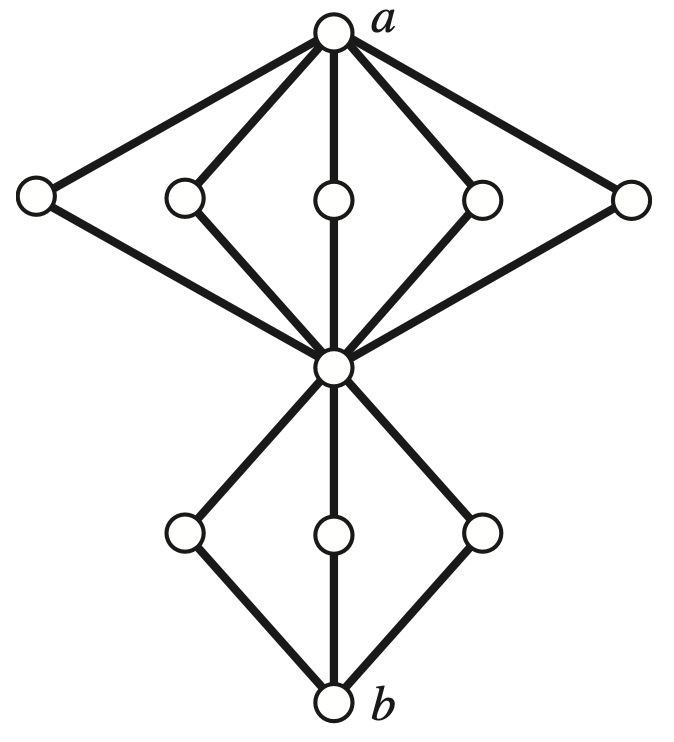
\includegraphics[width=.25\textwidth]{images/connection_exercise_1} %
\end{center}
\vfill 
\textbf{Solution.}
\begin{itemize}
\item[a.] There are 5x3=15 different paths from $a$ to $b$.
\item[b.] There are infinitely many walks from $a$ to $b$. To show this, it suffices to merely consider node $a$ and the node directly below it (which we'll call $c$).  We could bounce back and forth between these nodes however many times we'd like, and each would be a valid walk.  That is, possible walks include: $a \sim c, \; a \sim c \sim a, \;  a \sim c \sim a \sim c, \; a \sim c \sim a \sim c \sim a \; \cdots$.   
\end{itemize}

\end{frame}


\begin{frame}{Solution to group exercise \#2}
\small 
\noindent
\textbf{Problem.} Let $G$ be a graph.  A path $P$ in $G$ that contains all the vertices of $G$ is called a \textit{Hamiltonian Path}.  Prove that the graph in the bottom figure of the group exercises does not have a Hamiltonian path.

\vfill 
\textbf{Solution.}  Color the graph as follows.
\begin{center}
    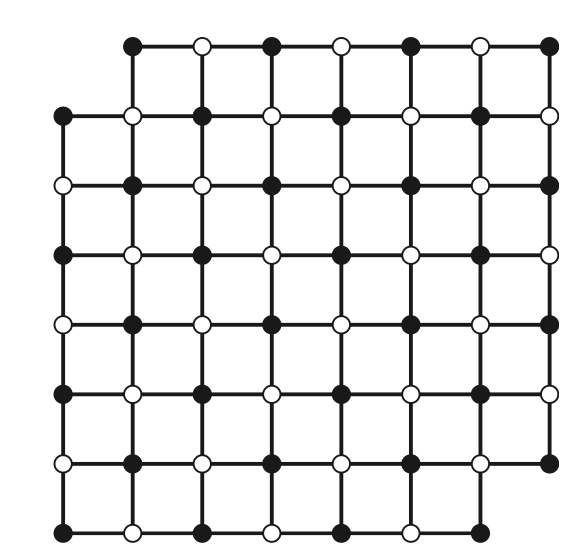
\includegraphics[width=.25\textwidth]{images/connection_hint} %
\end{center}

Suppose a Hamilton path $P$ exists.  We can think of $P$ as list of vertices where each one is adjacent to the next. However, note that neighbors of a white vertex are always black, and neighbors of a black vertex are always white.   Thus $P$ must alternate between black and white vertices.  Now, there are $2(3+5+7)=30$ white vertices and $2(2+4+6) + 8 = 32$ black vertices.  Hence, any enumeration of the 62 vertices must contain at least two consecutive vertices that have the same color. This is a contradiction. 
\end{frame}


\begin{frame}{Solution to group exercise \#3}
\small 
\textbf{Problem.} How many Hamiltonian paths does a complete graph on $n \geq 2$ vertices have?  
\vfill 
\textbf{Solution.} $n!$, since there are $n!$ ways to permute the $n$ vertices. 
\vfill 
\textbf{Remark.} Let's make the argument more concrete.  Let $K_n$ be the complete graph on $n$ vertices.  By enumeration, $K_2$ has two Hamiltonian paths: $a \sim b$ and $b \sim a$. Also by enumeration,  $K_3$ has six Hamiltonian paths: $a \sim b \sim c$, $a \sim c \sim b$,  $b \sim c \sim a$, $b \sim a \sim c$,  $c \sim a \sim b$, and $c \sim b \sim a$. For $K_4$, enumeration is starting to become unwieldy, so we think more abstractly: we have 4 choices for where to start ($a,b,c$ or $d$), then 3 choices of where to go next, then 2 choices for after that, and then the destination spot is determined.

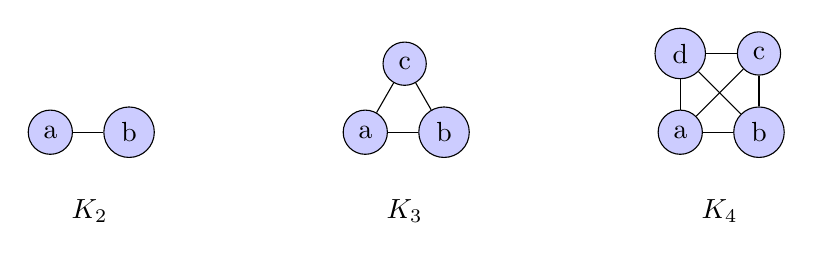
\begin{tikzpicture}[every node/.style={circle, draw, fill=blue!20, minimum size=0.5cm}]
    
    % K2
    \begin{scope}[xshift=0cm]
        \node (a1) at (0,0) {a};
        \node (a2) at (1,0) {b};
        \draw (a1) -- (a2);
		\node[draw=none, fill=none, shape=rectangle] at (0.5,-1) {$K_2$};
    \end{scope}
    
    % K3
    \begin{scope}[xshift=4cm]
        \node (b1) at (0,0) {a};
        \node (b2) at (1,0) {b};
        \node (b3) at (0.5,0.87) {c};
        \draw (b1) -- (b2);
        \draw (b2) -- (b3);
        \draw (b3) -- (b1);
        \node[draw=none, fill=none, shape=rectangle] at (0.5,-1) {$K_3$};
    \end{scope}
    
    % K4
    \begin{scope}[xshift=8cm]
        \node (c1) at (0,0) {a};
        \node (c2) at (1,0) {b};
        \node (c3) at (1,1) {c};
        \node (c4) at (0,1) {d};
        \foreach \i in {1,2,3,4} {
            \foreach \j in {1,2,3,4} {
                \ifnum\i<\j
                    \draw (c\i) -- (c\j);
                \fi
            }
        }
        \node[draw=none, fill=none, shape=rectangle] at (0.5,-1) {$K_4$};
    \end{scope}

\end{tikzpicture}

\end{frame}

\begin{frame}{Solution to group exercise \#4a}
\small 
\textbf{Problem.} Let $G$ be a graph with $n \geq 2$ vertices.   Prove that if G has at least $\binom{n-1}{2} +1$ edges, then $G$ is connected.
\vfill 

\textbf{Solution.}
 We proceed \colorbox{green!30}{by contraposition}.  Suppose $G$ is not connected. Then there is a vertex $v$ not connected to any other vertex.  Thus, there must be at least $n-1$ edges missing from the maximum possible number $\binom{n}{2}$.  That is, there can be no more than $\binom{n}{2} - (n-1)$ edges.  But
    %
    \begin{align*}
    \binom{n}{2} - (n-1) &= 	 \binom{n}{2} -   \binom{n-1}{1} \\
    &= \binom{n-1}{2} && \text{\colorbox{red!30}{\footnotesize{(By Pascal's Identity)}}}
    \end{align*}
    %
    So there are at most $\binom{n-1}{2}$ edges.
\vfill 
\colorbox{green!30}{\textbf{Remark 1.}} Recall that a \colorbox{green!30}{proof by contraposition} proves $A \implies B$ by proving $\lnot B \implies \lnot A$.
\vfill 
\colorbox{red!30}{\textbf{Remark 2.}} From \colorbox{red!30}{Pascal's identity}, we have
\[\binom{n}{2} = \binom{n-1}{1}  + \binom{n-1}{2}  \]
\end{frame}

\begin{frame}{Solution to group exercise \#4b}

\textbf{Problem.} Show that the result in \#4a is best possible; that is, for each $n \geq 2$, prove there is a graph with 	$\binom{n-1}{2}$ edges that is not connected.
\vfill 

\textbf{Solution.}
    \begin{itemize}
        \item[b.] Select any vertex (we'll call it $v^*$) to isolate.  Of the remaining $n-1$ vertices, form the complete graph $K_{n-1}$.  The subgraph $K_{n-1}$ has $\binom{n-1}{2}$ edges.  However, the full graph $G$ is disconnected, since there is no path that connects $v^*$ to any other vertex.  
    \end{itemize}
\end{frame}

\begin{frame}[standout]
Appendix	
\end{frame}

\begin{frame}
%\small 

\begin{mygreenbox}[title=\text{Practice reading quiz (Connection)}]

The argument below is from the text.  Is it right or wrong?  If it's wrong, what is the problem with it?
\end{mygreenbox}
\vfill 
\begin{myyellowbox}[title=\text{Reference passage from text}]
\begin{minipage}{.68\textwidth}
Is the is-connected-to relation transitive? Suppose, in a graph $G$, we know that $x$ is connected to $y$ and that $y$ is connected to $z$.  We want to prove that $x$ is connected to $z$. \\
\vspace{.15cm}

Since $x$ is connected to $y$, there must be an $(x,y)$-path; let's call it $P$.  And since $y$ is connected to $z$, there must be a $(y,z)$-path.  Let's call it $Q$.  Notice that the last vertex of $P$ is the same as the first vertex of $Q$ (it's y).  Therefore, we can form the concatenation $P+Q$, which is an $(x,z)$-path.  Therefore $x$ is connected to $z$.
\end{minipage} %
\hfill 
\begin{minipage}{.28\textwidth}
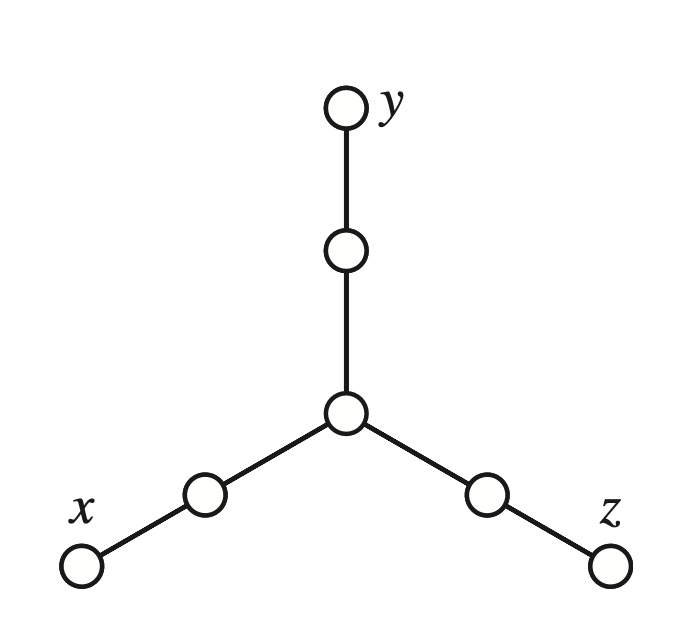
\includegraphics[width=\linewidth]{images/transitivity_of_connection.png}
\end{minipage}

\end{myyellowbox}

\end{frame}




\end{document}
